\section{Yield data}
For our yield data, we make use of the dataset published by~\textcite{gurkaynak_us_2007}. 
This dataset consists of United States Department of Treasury zero-coupon, continuously compounded, yield curve data. 
The dataset contains daily yield curve data from the 14th of June 1961 to the 1st of May 2020, at the time of writing. 
This dataset contains maturities from 1 year up to and including 30 years. 
For our research only the maturities from 1 year up to and including 10 years are used. 
Because yield curve estimates only extended out to 7 years until the 16th of August 1971~\parencite[see][p.~19]{gurkaynak_us_2007}, our sample will start from August 1971 to December 2016. 

\section{Macroeconomic data}
For our macroeconomic data, used for constructing the (macro-)factors, we make use of the FRED-MD dataset, published by~\textcite{mccracken_fred-md_2016}. 
This dataset is developed by the United States Federal Reserve Bank of St. Louis and consists of 134 monthly U.S. macroeconomic variables from January 1959 to March 2020, at the time of writing. 
By deleting all variables containing blank cells, only 105 variables remain. 
We make use of the same sample as the yield data.

\section{Samples}
\label{sec:samples}
For our research, we use the following samples to compare our various different models:
\begin{enumerate}
	\item Subsample 1, January 1992 to December 1999, this is our pre-dot-com bubble crash sample,
	\item Subsample 2, January 2000 to December 2007, this is our dot-com bubble crash and 9/11 sample leading up to the great recession,
	\item Subsample 3, January 2008 to December 2016, this is our (post-)great recession sample,
	\item Full sample, January 1992 to December 2016.
\end{enumerate}
These samples roughly correspond to the samples used by~\textcite{swanson_big_2017}. Surface plots of these samples are given in~\cref{fig:samples}. 

\begin{figure}
     \centering
     \begin{subfigure}[b]{0.45\textwidth}
         \centering
         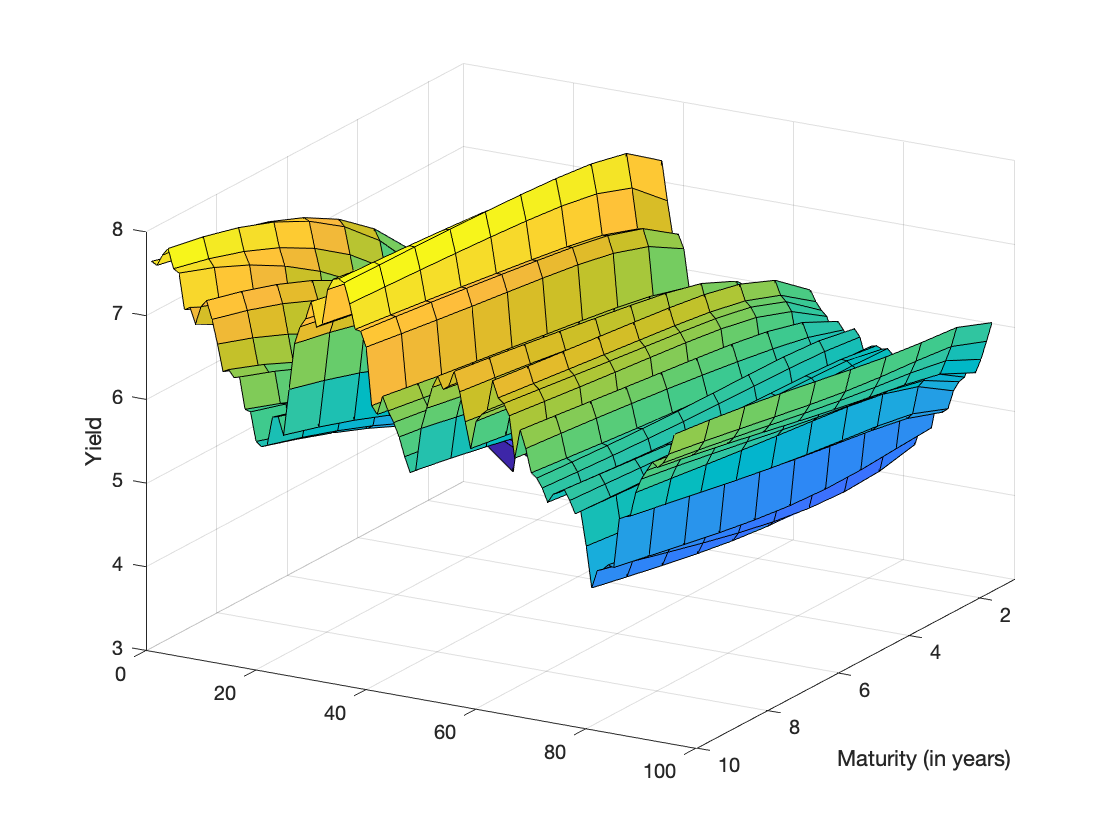
\includegraphics[width=\textwidth]{figures/sample1}
         \caption{Subsample 1}
         \label{fig:subsample1}
     \end{subfigure}
     \begin{subfigure}[b]{0.45\textwidth}
         \centering
         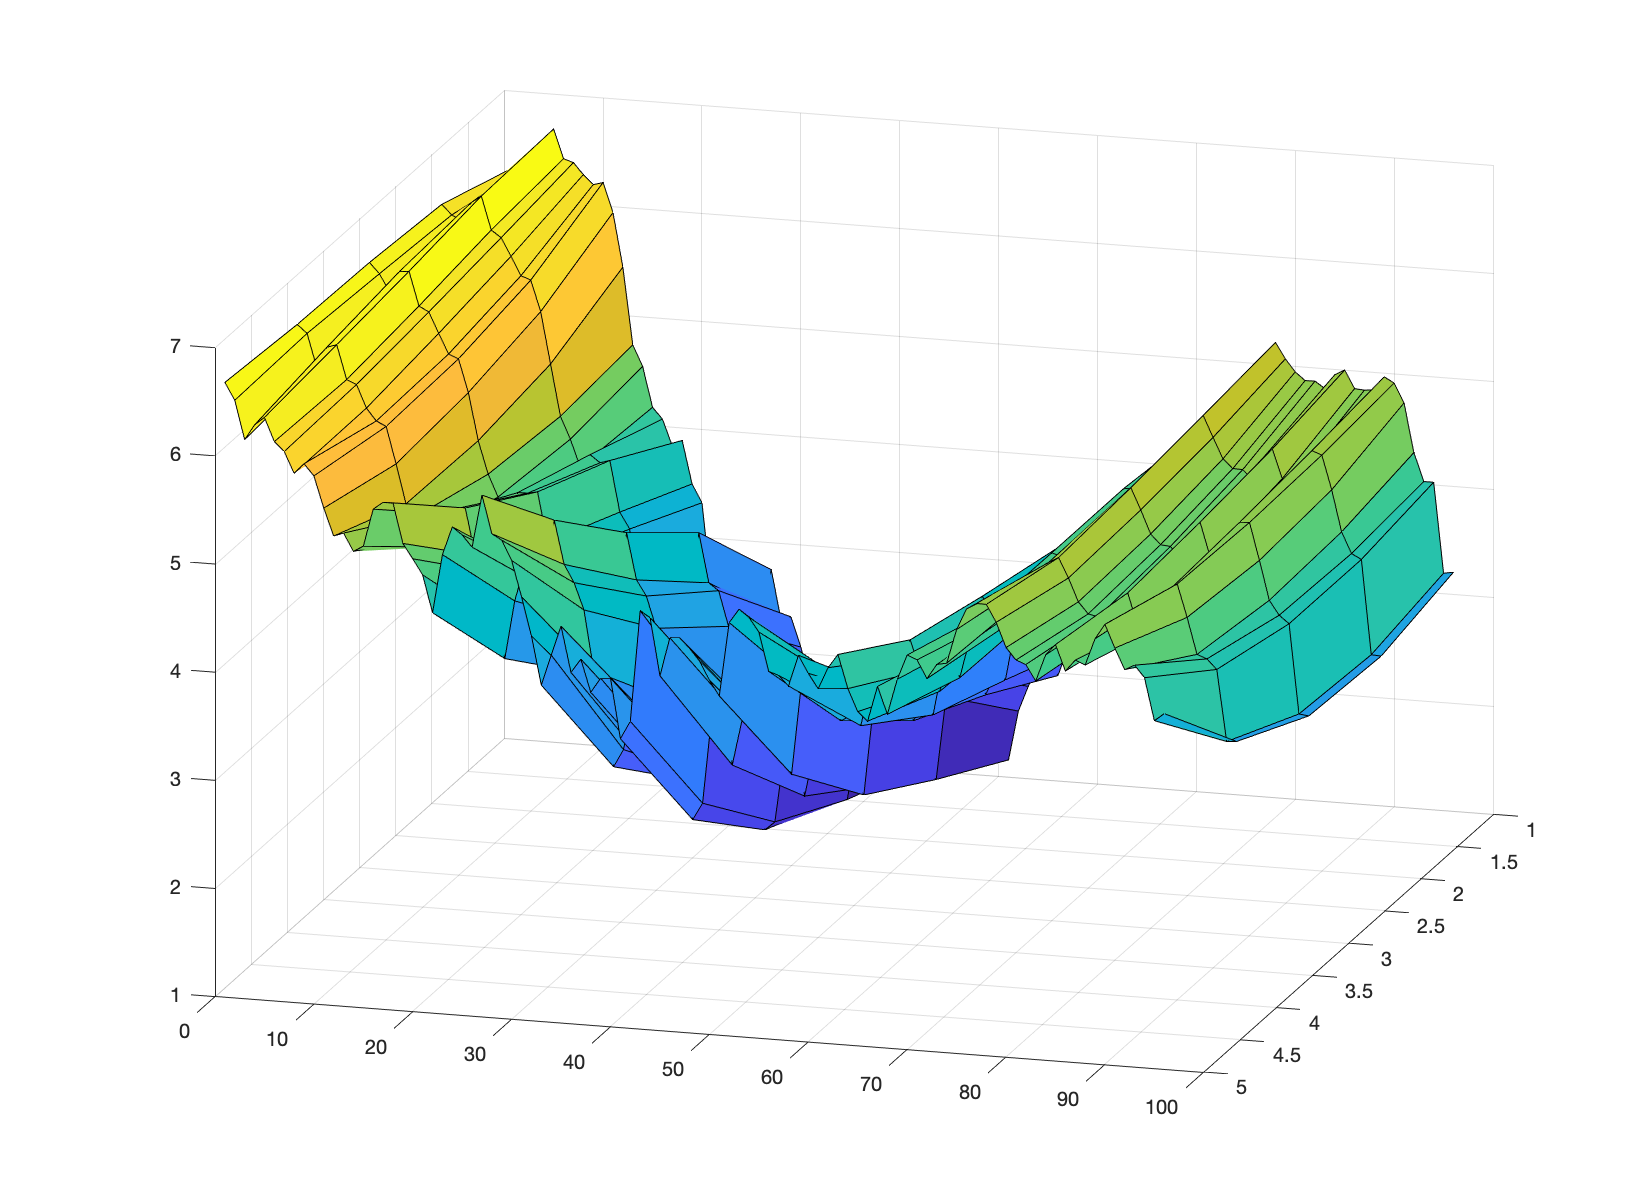
\includegraphics[width=\textwidth]{figures/sample2}
         \caption{Subsample 2}
         \label{fig:subsample2}
     \end{subfigure}
     \begin{subfigure}[b]{0.45\textwidth}
         \centering
         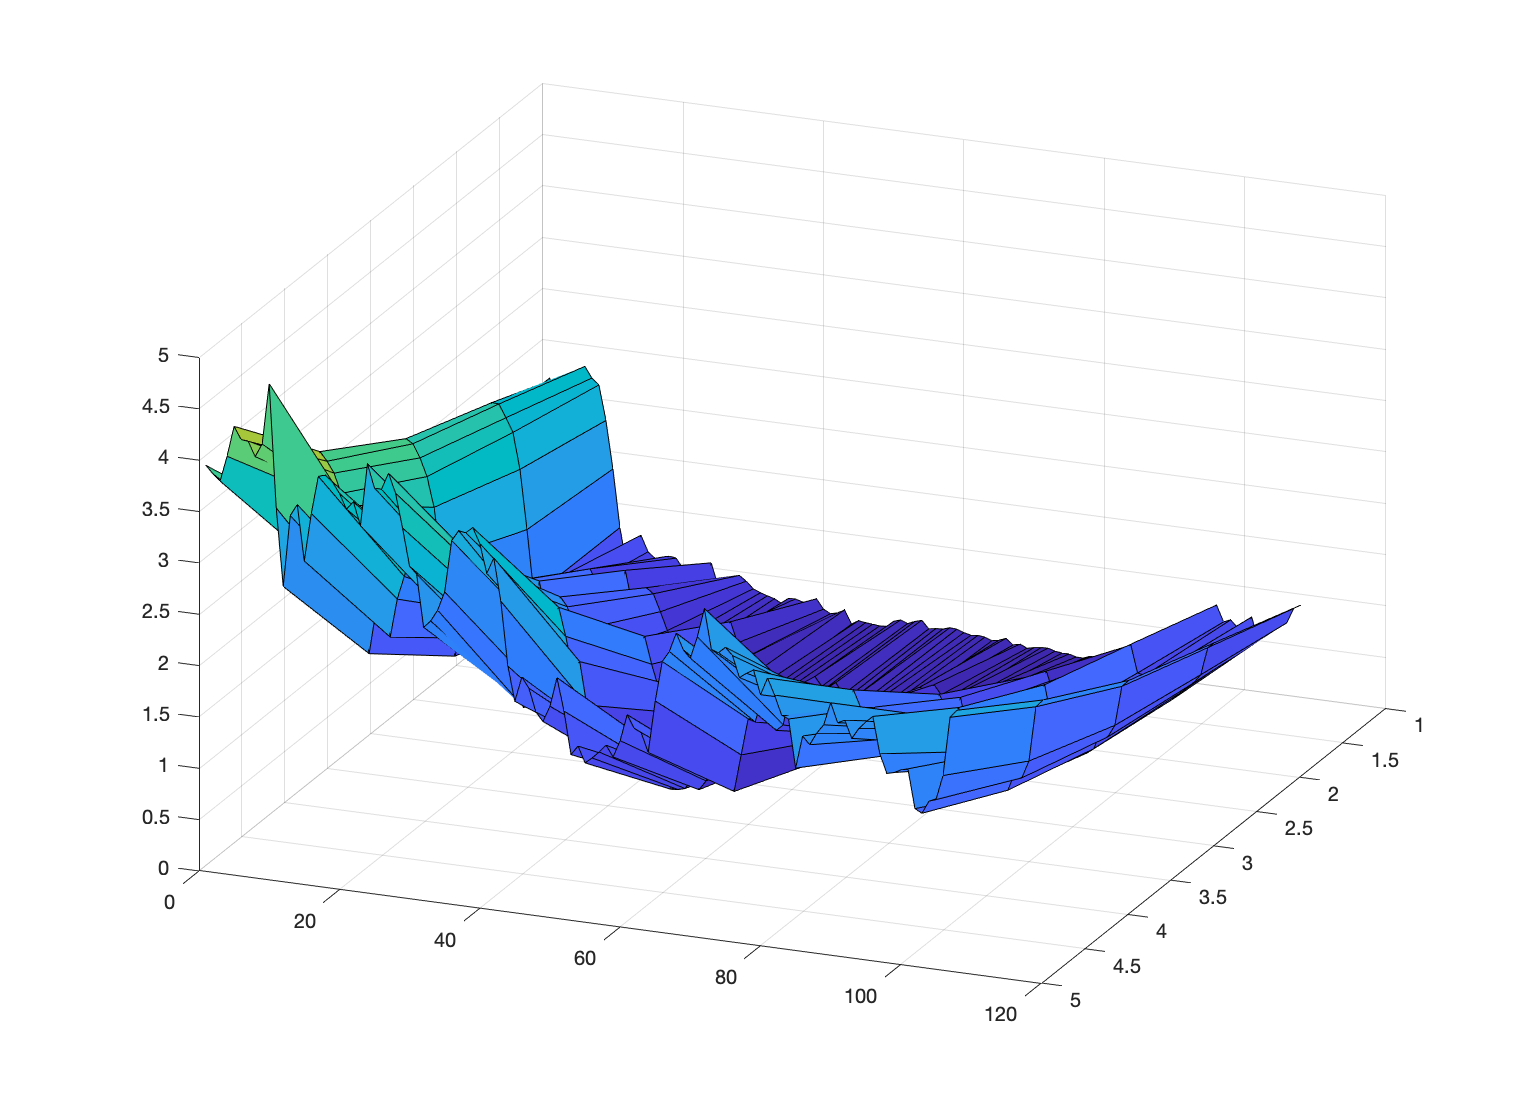
\includegraphics[width=\textwidth]{figures/sample3}
         \caption{Subsample 3}
         \label{fig:subsample3}
     \end{subfigure}
     \begin{subfigure}[b]{0.45\textwidth}
         \centering
         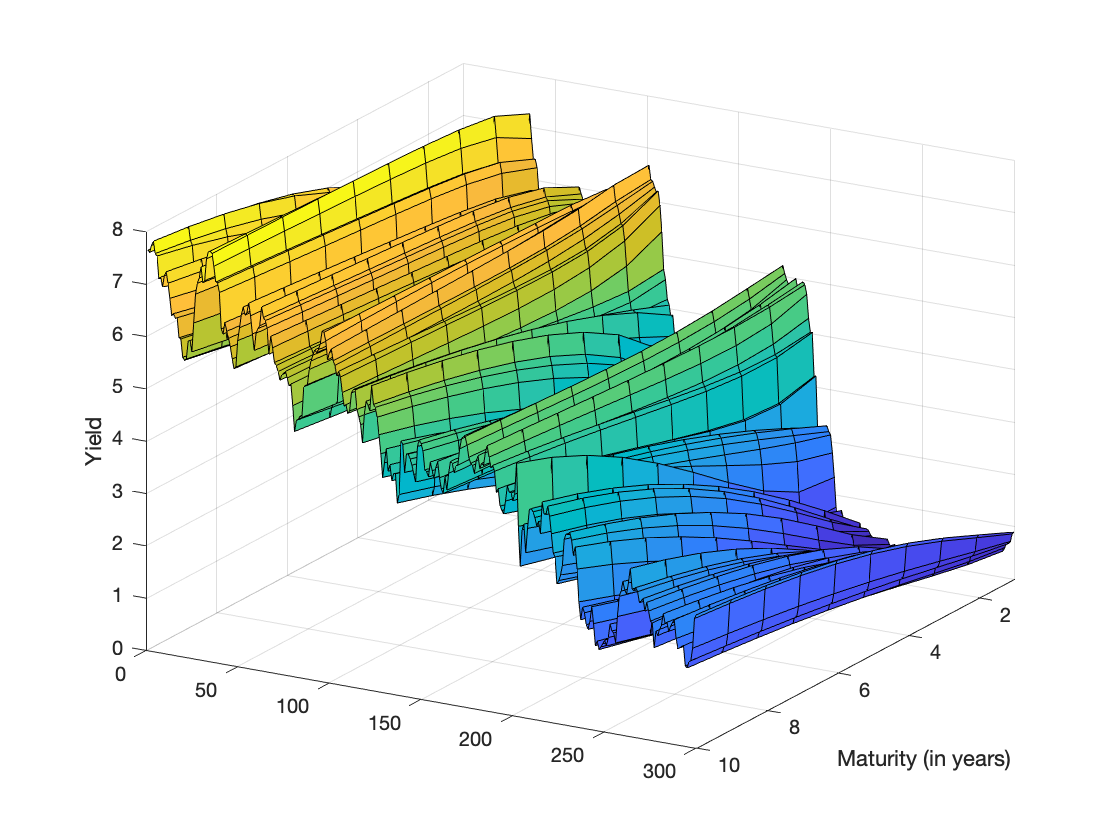
\includegraphics[width=\textwidth]{figures/fullsample}
         \caption{Full sample}
         \label{fig:fullsample}
     \end{subfigure}
     \caption{Surface plots of the 4 different samples}
     \label{fig:samples}
\end{figure}